\hoofdstuk {Methodology}

\paragraaf{Research method}

The method applied for researching the problems of this project and its possible solutions is called \emph{literature review}. This method consists of researching what has already been published, which might be in the form of scientific or engineering papers, journals, thesis, etc., by accredited scientists, scholars or engineers concerning this assignment's topics. 
This method is applied for searching for potential algorithms which can be used to solve the problems facing the project. Once a group of the most suitable algorithms has been found, the best one must be chosen and the reasoning for this choice must be explained. When the choice has been made, the algorithm can then be implemented using the chosen development method.

\paragraaf{Development method}

This project will be developed using the \emph{Iterative Application Development} (IAD) method. This development method works by dividing the project into smaller `sub-projects', called \emph{cycles}, and incrementing them to past cycles, which will ultimately lead to a complete system. Each cycle consists of three phases, which can be repeated multiple times if necessary, called \emph{iterations}. These iterations are: \emph{definition}, \emph{development} and \emph{deployment}.

During the definition phase the goals, limitations and conditions for the current cycle are examined and described. If a previous cycle has been completed, it will be evaluated during this phase. This phase is intended for thinking towards the completion of the project and to achieve a more clear picture of the system as a whole.
After defining the objective for the new cycle, the software will be developed. After finishing, the software is then integrated with the software developed in the previous cycles and becomes therefore part of the general project.

This method of software development brings multiple benefits: The complexity of the project is decreased by breaking down the problem into smaller chunks, which allows for faster and more concrete results and makes it therefore easier to get better feedback or to solve critical bottlenecks by being able to discuss them at the end of each cycle. The project development also becomes more flexible by having the possibility to review the requirements and strategies every cycle.

Each cycle lasts 2 weeks and at the end of each cycle the evaluation of the past cycle and the objective for the coming cycle will be discussed with the organisation's mentor.

\hoofdstuk{Algorithms}

\paragraaf{Plate localization}

When searching for possible algorithms which make it possible to find license plates in an image, two main types came forth from the research: feature detection and edge detection. 

The feature detection algorithms works by finding so called \emph{features} in a image, which are used to recognize the first image within a second one. These features are segments of an image which must be uncommon, as to reduce the possibility of retrieving a false positive when applying the algorithm, and also consist of something which can be objectively described to a computer. Because of these requirements, the features extracted from an images are usually corners since corners usually only match themselves when compared to other segments in an image. This opposed to flat surfaces or lines, which may appear multiple times in multiple places in the same image. Because this algorithm focuses on detecting the uniqueness of an image and using those attributes to detect themselves in different images, it is difficult to use feature detection for the recognition of license plates for the reason that every license plate contains unique text. The considerable collection of diverse shapes that exist in the Latin alphabet create false positives which are often detected in random and incorrect locations. One possible approach to use this algorithm would be by creating a feature database of every possible alphanumeric character and then finding the highest concentration of text as a possible location. 

The other possible algorithm is mostly based on edge detection. This kind of algorithm works by applying an edge detection filter to a grey scale version of the image where the car is present, e.g. the Sobel Filter [ref here] or Canny Edge Filter [ref here]. This creates a binary image where the edges of every shape present in the image are displayed. Because of the nature of one of the characteristics common to every license plate, which is the presence of text, an area with a high density of edges is created. Although license plates are not the only objects which might have such a property, e.g. a fence, it is the most common one which might be encountered while driving. By applying this filter to find horizontal edges it is possible to find the vertical location of the plate and then vice-versa to find the horizontal location and by extension the plate itself. Due to little information on the performance of the first algorithm and an healthy amount of information regarding this one, this algorithm was chosen.

\paragraaf{Text recognition}

\textbf{`Explanation on training Tesseract'}

\hoofdstuk{Design}

Because the application implemented is an Android application, its design was created with Android's design rules in mind. A flowchart illustrating the general design and flow of the application is displayed in Figure \ref{fig:architecture}. Within an Android application all components run in the same thread by default, which is also known as the `main thread', and is identified in the flowchart as `UI' because it is used mainly to regulate all the processes related to the user interface. One of those processes, and also one of the most fundamental running in this thread, is the process which captures images from the device's camera. The process captures image frames at a set rate in order to avoid the unnecessary capture of very similar images and, because image processing algorithms consist of a large number of calculations and therefore might take a long time to finish, to avoid overwhelming the application with too many frames. These images are then pushed into a buffer, called `Frames buffer', where they are kept until they are able to be processed. For the same reasons the camera only captures frames at a specific rate, this buffer has a limit of how many frames can be stored within but with the intention of only preserving images which are as recent as possible, before a new frame is added the oldest remaining frame in the buffer is removed. This process runs until the application is terminated.

As explained before, image processing is rather heavy and it is necessary to use every tool available to increase the application's performance. One of these tools is multi-threading and apart from the UI thread this application uses two other kinds of threads, up to a total of four threads which is also the number of physical cores in the used device and therefore gives every thread a dedicated core. The processes called `Find bands' and `Find plate' use a type of thread called a \emph{One-Call Thread}, which are threads used for a short period of time and only run when called. The other kind of thread is called a \emph{Permanent thread}. This type of thread is started during the initiation of the application, runs parallel to the UI thread and lives as long as the application itself. This process is responsible for checking whether the bands and plates buffers have available items and for calling the respective processes to process them. Further, if a plate is found then this thread applies text recognition to retrieve the displayed text and tries to match it with the database entries. 

\textbf{`add database and database entries retrieval'}

\figuur{width=\textwidth}{plaatjes/architecture-RoadEye-parallel.png}{architecture}{System flow diagram}

% --------------------------------------------------------------------------------------------------------------------------------------------------------------

\hoofdstuk{Implementation}

The application consists of three important components: the algorithm for finding the vertical location of the license plates, the plate localization algorithm and the text recognition component. Both localization algorithms are based on the of \textbf{`Java ANPR add ref here'}, with some slight deviation on the methods used. The car in Figure \ref{fig:car-source} is used to demonstrate how the algorithm works.

\paragraaf{Bands}

The first step to finding a license plate is to find its vertical location, which also known as a band. By making use of one of the most characteristic features of a Dutch license plate, which is its yellow colour and can be seen on Figure \ref{fig:dutch-plate}, it is possible to reduce the area of the image where the license plate might be located through the application of colour segmentation. 


\figuur{width=0.3\textwidth}{plaatjes/dutch-plate}{dutch-plate}{Dutch license plate.}

Colour segmentation consists of grabbing only the areas of an image which fall within a specified range and is usually used on an image which uses the HSV colour space representation. As seen in Figure \ref{fig:hsv}, HSV stands for Hue, Saturation, and Value and it is a way of representing colours on a computer. This in contrast to the most widely used colour space, the RGB colour space (Red, Green, Blue) which uses a combination of three different colours to represent a specific colour, the HSV colour space uses the H-value to represent the colour and is defined in degrees (0$^{\circ}$ - 360$^{\circ}$), the S-value to represent how bleak or how colourful the colour is and is defined with a percentage (0\% - 100\%), and the V-value to represent how bright or dark a colour is and is defined the same way as the saturation. This provides a system where it is simple to specify a range of colour for the colour segmentation algorithm. The range chosen for the license plate lays between 40$^{\circ}$ and 50$^{\circ}$, which is broad enough to take into consideration the deviations in the colour of the plate caused by shadows and reflections.

\figuur{width=0.3\textwidth}{plaatjes/hsv}{hsv}{HSV colour space.}


As a result of segmenting the yellow colour from the source image, the image in Figure \ref{fig:color-segmented} is created and it is quite visible where the plate is located. \textbf{`part about removing the small speckles'}. Because there are such things as yellow cars and other yellow objects everywhere, an extra step must be taken to increase the chance of finding plates instead of some random object. This is accomplished by making use of a characteristic of text and by extension of license plates, which is a high number of edges. By applying an edge detection algorithm, which in this case is the Sobel algorithm \textbf{`add ref here'} and the results are visible in Figure \ref{fig:edge-detected}, we still get a visible area where the plate is located but in case the source image contained large yellow areas, these areas are now mostly gone. 

Once that is done, the application can start analysing the previous image for a possible location of the license plate. This is done by summing up the intensity of every pixels on each row, therefore creating a graph of the density of edges on each row. Before making any decisions concerning the location of the plate on the graph, a filter must be applied to the data to decrease the chance of retrieving a wrong area of the image. This filter is called a \emph{mean-filter} and works by summing up the values of a specific number of the previous and next data values, in the case of this application seven values are used, with the current value and by diving it by the total number of values. The results in the `smooth' graph displayed in Figure \ref{fig:possible-bands}. The next step and last step is finding the potential plate areas and this is done by finding a number of the highest peaks in the graph, with three being the default. The reason for trying to find multiple areas, is in case an object on the image happens to have a higher edge density than the plate and therefore increasing the chance of still finding it. The way the application finds peaks, is by finding the highest value in the data set and then searching for the right and left boundary of the peak by iterating towards its respective side until it finds a value which equal to or smaller than 10\% of the highest value of the peak. The coordinates of both boundaries are then saved and the area in between both boundaries is made equal to zero, or \emph{zeroized}. By rinsing and repeating this process for the desired number of peaks, the bands are found and the images such as the ones also displayed on Figure \ref{fig:possible-bands} are created. 

\begin{figure}[h]
        \centering
        \begin{subfigure}{0.37\textwidth}
            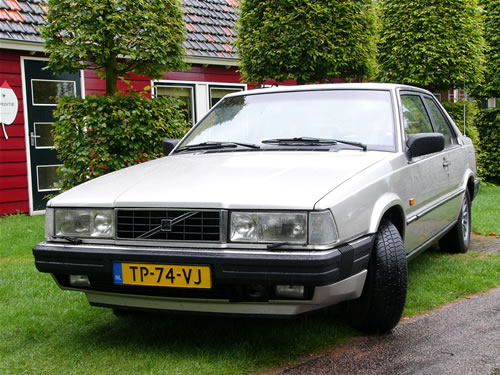
\includegraphics[width=\textwidth]{plaatjes/car}
            \caption{Source car image.}
            \label{fig:car-source}
        \end{subfigure}%
       	~ 
        \begin{subfigure}{0.3\textwidth}
            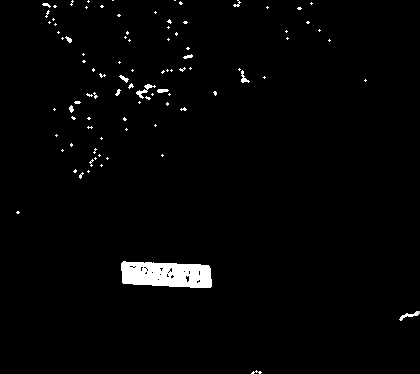
\includegraphics[width=\textwidth]{plaatjes/yellow-segment}
            \caption{Yellow segmentation of source image.}
            \label{fig:color-segmented}
        \end{subfigure}%
        ~ 
        \begin{subfigure}{0.33\textwidth}
            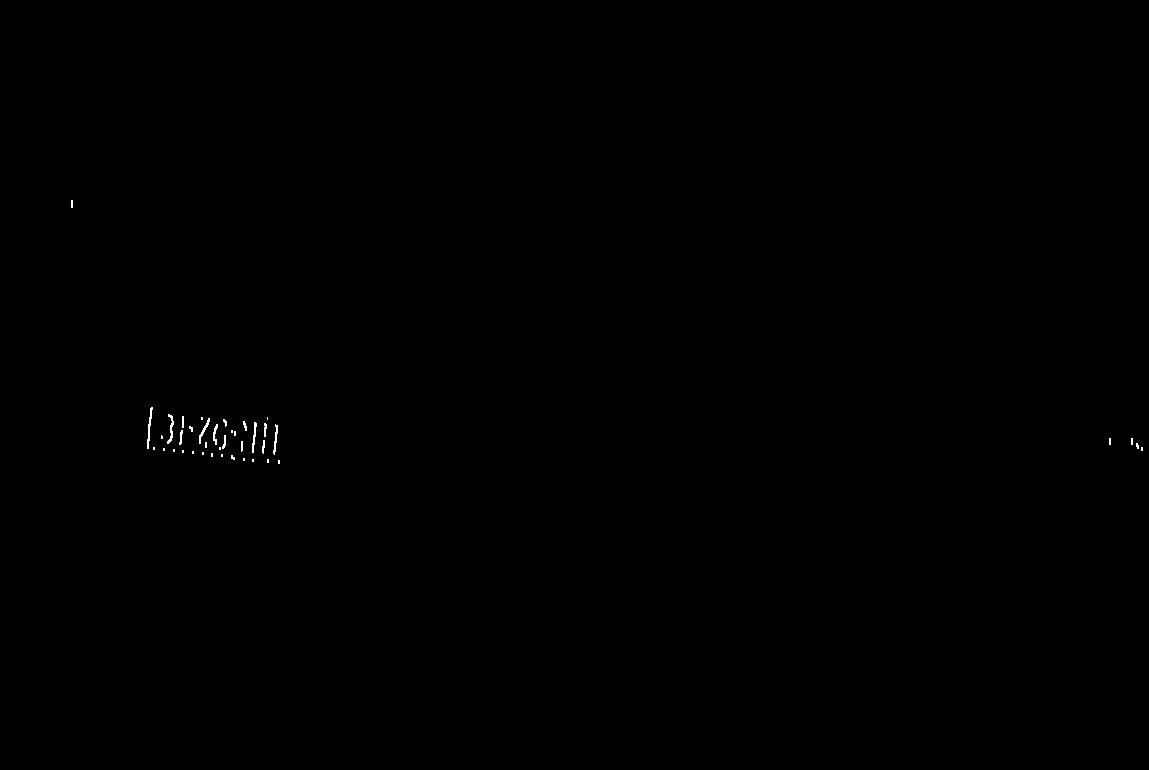
\includegraphics[width=\textwidth]{plaatjes/edge-detection}
            \caption{Edge detection.}
            \label{fig:edge-detected}
        \end{subfigure}%

        \begin{subfigure}{0.5\textwidth}
            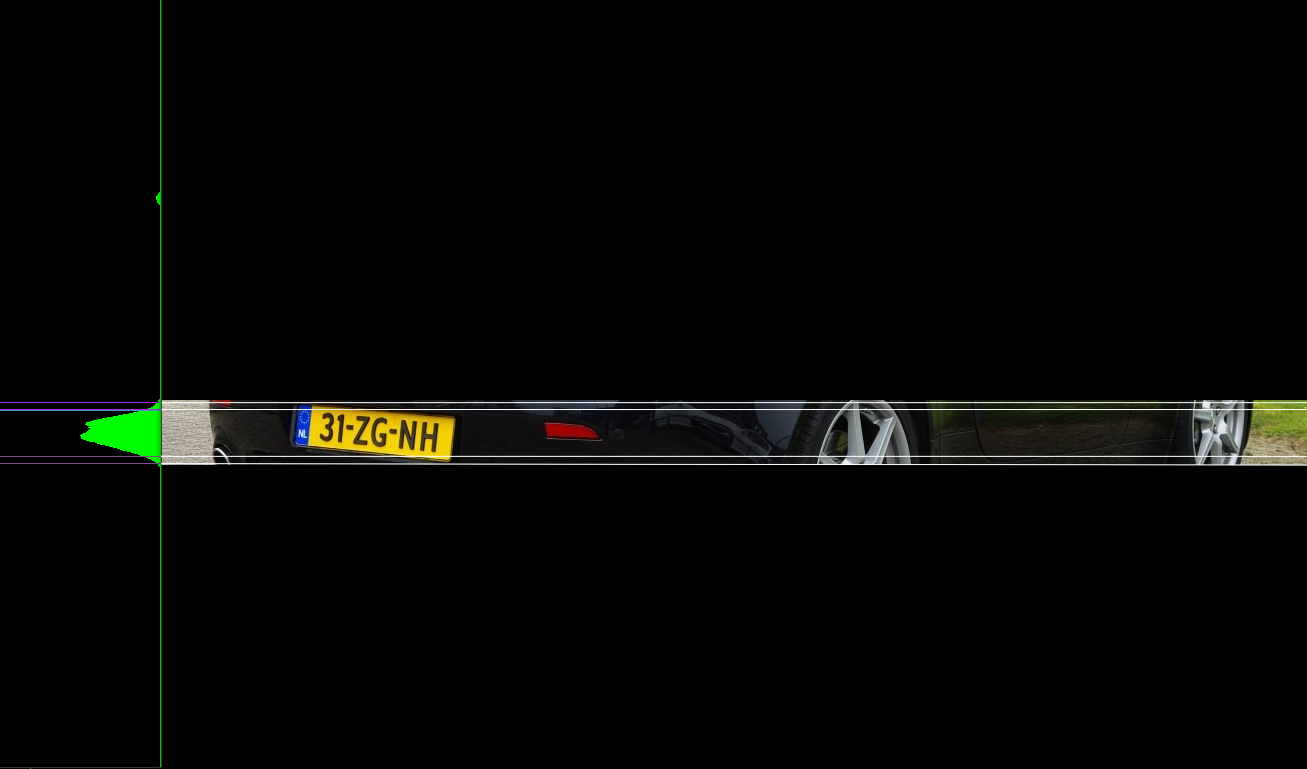
\includegraphics[width=\textwidth]{plaatjes/3-peaks}
            \caption{Three possible bands.}
            \label{fig:possible-bands}
        \end{subfigure}%

        \caption{Phases from band localization.}
        \label{fig:find-band}
\end{figure}

\paragraaf{Plates}


